\documentclass[12pt, a4paper]{report}

% Импорты 
\usepackage{cmap}
\usepackage{url}
\usepackage{hyperref}
\usepackage{amsthm, amsmath, amssymb}
\usepackage{thmtools}
\usepackage{fancyhdr}
\usepackage{graphicx}
\usepackage{titlesec}
\usepackage[normalem]{ulem}

\usepackage[english, russian]{babel}
\usepackage[utf8]{inputenc}
\usepackage[T2A]{fontenc}

% Геометрия 
\usepackage{geometry}
\geometry{
	left=1.5cm,
	right=1.5cm,
	top=2cm,
	bottom=1.5cm
}
\setlength\parindent{0pt}

% Теоремы, леммы ...
\renewcommand{\listtheoremname}{Список теорем}

\newtheorem{theorem}{Теорема}[section]
\newtheorem{lemma}[theorem]{Лемма}
\newtheorem{corollary}[theorem]{Следствие}
\theoremstyle{definition}
\newtheorem*{definition}{Определение}
\theoremstyle{remark}
\newtheorem{remark}[theorem]{Замечание}
\newtheorem{example}[theorem]{Пример}

% Колонтитулы
\pagestyle{fancy}
\fancyhf{}
\fancyhead[R]{\rightmark}
\fancyhead[L]{\textsc{\thechapter. \leftmark}}
\fancyfoot[C]{\thepage}
\renewcommand{\chaptermark}[1]{\markboth{#1}{}}
\renewcommand{\sectionmark}[1]{\markright{#1}}

% Главы
\titleformat{\chapter}[display]
{\normalfont\huge\bfseries\centering} % Формат текста
{\titlerule[1pt] \vspace{1pt} \titlerule\vspace{1pc} \Huge\MakeUppercase{\chaptertitlename} \thechapter} % Номер главы
{1pc} % Отступ между номером главы и названием
{\Huge} % Формат названия главы
[\vspace{1pc} \titlerule] % Декоративные элементы после названия

\titlespacing*{\chapter}{0pt}{0pt}{40pt}

\begin{document}
	
	\begin{titlepage}
		\newgeometry{left=1.5cm, right=1.5cm, top=3cm, bottom=2cm}
		\centering
		
		{\Large Санкт-Петербургский губернаторский\\ Физико-математический лицей №30}\\[1cm]
		
\includegraphics[width=0.18\textwidth]{assets/logo.png}\\[5cm]
		
		\textbf{ \LARGE Конспект важных уроков N-го класса}\\[2cm]
		
		\begin{flushright}
			\textbf{Ученика:} \\ Идеалова Идеала \\[1cm]
			\textbf{По мотивам уроков:} \\ Лучшего учителя на свете \\[1cm]
		\end{flushright}
		
		\vfill
		
		{\large 2023--2024 г.}
		
	\end{titlepage}
	
	\begin{abstract}
	
		Пример аннотации. 
		Lorem ipsum dolor sit amet, consetetur sadipscing elitr, sed diam nonumy eirmod tempor invidunt ut labore et dolore magna aliquyam erat, sed diam voluptua. 
		At vero eos et accusam et justo duo dolores et ea rebum. 
		Stet clita kasd gubergren, no sea takimata sanctus est Lorem ipsum dolor sit amet. 
		Lorem ipsum dolor sit amet, consetetur sadipscing elitr, sed diam nonumy eirmod tempor invidunt ut labore et dolore magna aliquyam erat, sed diam voluptua. 
		At vero eos et accusam et justo duo dolores et ea rebum. 
		Stet clita kasd gubergren, no sea takimata sanctus est Lorem ipsum dolor sit amet. \\
		
		\begin{center}
			*Какой-то мотивационный текст*
		\end{center} 
		
	\end{abstract}

	\newgeometry{left=1.5cm, right=1.5cm, top=1cm, bottom=2cm}
\tableofcontents
\setcounter{page}{0} 
\thispagestyle{empty}
\restoregeometry
	
	\chapter{Пример главы}

\section{Пример секции}

\begin{definition}
	Мир, это когда нет войны
\end{definition}

\begin{corollary}
	Где война нет мира
\end{corollary}


\begin{example}
	Пример примера
\end{example}

\begin{theorem}[О крокодиле]
	Крокодил более желтый, чем широкий
\end{theorem}

\begin{proof}
	Взгляните на крокодила, все станет понятно
\end{proof}

\begin{remark}
	Крокодил желтый только снизу, сверху он зеленый
\end{remark}

\begin{figure}[h]
    \centering
    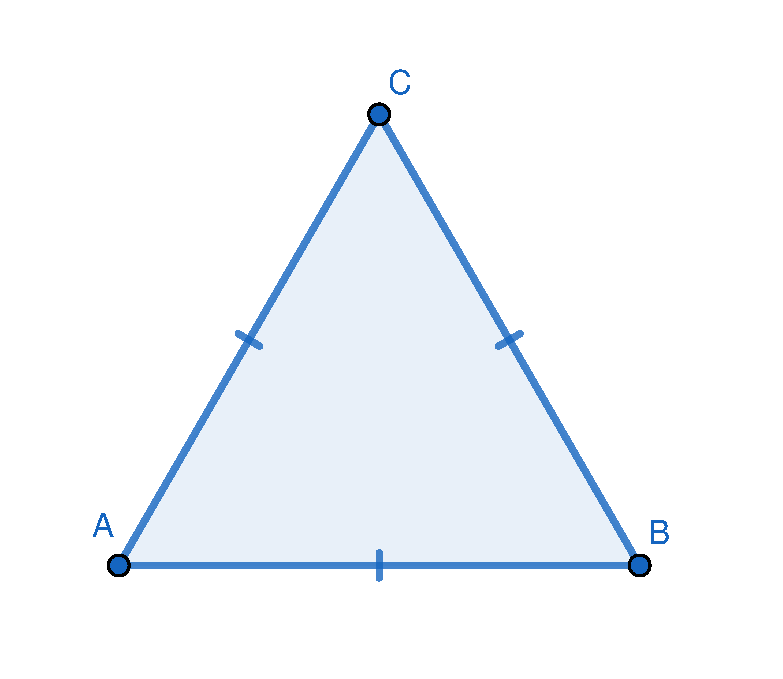
\includegraphics[height=5cm]{tex/chapter_1/assets/geogebra-export.pdf}
    \caption{Равносторонний треугольник}
\end{figure}



\end{document}

